% Figura do Cap. I: retroalimentação da variância no GARCH(1,1). Substitui o PNG
% antigo em 27/10/2026, a pedido do autor (alternativa G1, "Duas entradas, uma
% saída", de notas/rascunhos/diagramas_2026-10-27/alternativas.pdf). A constante
% omega fica fora do desenho, o texto a explica. Compilada pelo Makefile do tg/.
\documentclass[11pt,border=2pt]{standalone}
\usepackage[T1]{fontenc}
\usepackage[utf8]{inputenc}
\usepackage{mathptmx}
\usepackage{tikz}
\usetikzlibrary{arrows.meta,positioning}
\tikzset{
  seta/.style={-{Stealth[length=2.2mm]}, semithick},
  caixa/.style={rectangle, draw, semithick, fill=gray!10, rounded corners=2pt,
                align=center, minimum width=56mm, minimum height=9mm, font=\small},
  rotulo/.style={font=\footnotesize\itshape, align=center},
}
\begin{document}
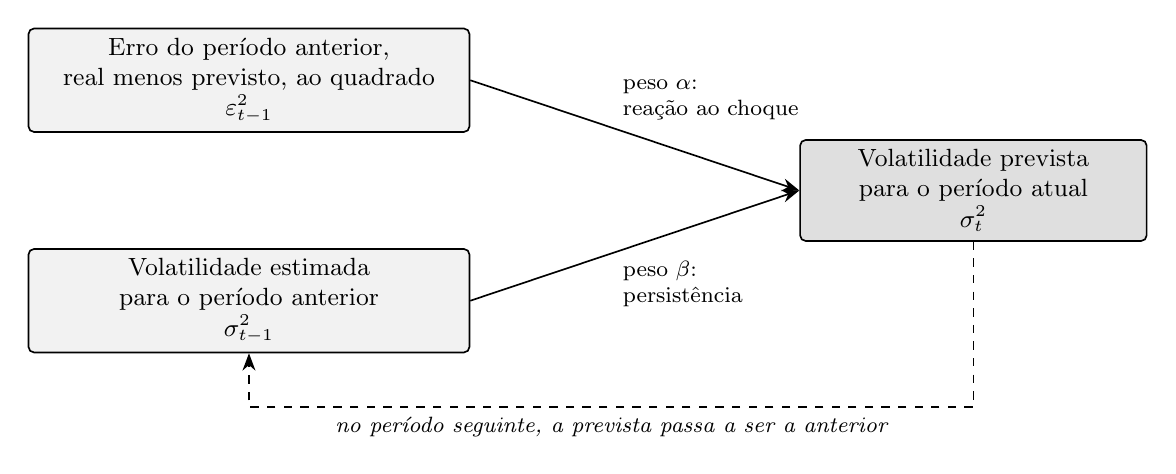
\begin{tikzpicture}
  \node[caixa] (ep) at (0,1.4) {Erro do período anterior,\\real menos previsto, ao quadrado\\$\varepsilon^2_{t-1}$};
  \node[caixa] (si) at (0,-1.4) {Volatilidade estimada\\para o período anterior\\$\sigma^2_{t-1}$};
  \node[caixa, minimum width=44mm, fill=gray!25] (out) at (9.2,0) {Volatilidade prevista\\para o período atual\\$\sigma^2_t$};
  \draw[seta] (ep.east) -- node[above right=0pt and -2pt, pos=0.45, font=\footnotesize, align=left]{peso $\alpha$:\\reação ao choque} (out.west);
  \draw[seta] (si.east) -- node[below right=0pt and -2pt, pos=0.45, font=\footnotesize, align=left]{peso $\beta$:\\persistência} (out.west);
  \draw[seta, dashed] (out.south) -- ++(0,-2.1) -| (si.south)
    node[pos=0.25, below, rotulo]{no período seguinte, a prevista passa a ser a anterior};
\end{tikzpicture}
\end{document}
